% cite JDemetra+
% find more about survey
    % sampling
    % questions (no change?)
    %


% ----------- Cover Master Thesis Faculty of Sciences ---------------
% This document should be compiled with pdflatex.  If you want to use
% latex to compile to dvi/ps, you have to convert the images to (e)ps
%                           -- December 2012
% -------------------------------------------------------------------
\RequirePackage{fix-cm}
\documentclass[12pt,a4paper,oneside]{book}


% ------------------------- Load packages ---------------------------
% You can eventually add these while you load other packages
% in case you want to integrate the titlepage with the rest of your thesis
% -------------------------------------------------------------------
\usepackage{graphicx,xcolor,textpos}
\usepackage{helvet}
\usepackage{multirow}

\usepackage[colorlinks=true ,citecolor=blue, linkcolor=black]{hyperref}
\usepackage{csquotes}
\usepackage[comma]{natbib}
%\bibliographystyle{apa}
\usepackage{amsmath}
\usepackage{mathtools}

\usepackage{lipsum}

\providecommand{\keywords}[1]{\textbf{\textit{Keywords:}} #1}

%\setcounter{tocdepth}{2}% Allow only \chapter in ToC

\usepackage[Sonny]{fncychap} % chapter style

\usepackage{listings} % cite R code

\usepackage{graphicx} 
\usepackage{fancyvrb} 

\usepackage{import}
\usepackage{subfiles}

\usepackage{float}

\usepackage{dcolumn}

\usepackage{subcaption}

\usepackage{wrapfig}

\usepackage{pdflscape}

\usepackage{wasysym}

\usepackage{pgfplots}
\pgfmathdeclarefunction{gauss}{2}{%
  \pgfmathparse{1/(#2*sqrt(2*pi))*exp(-((x-#1)^2)/(2*#2^2))}%
}

\lstset{% setup listings 
        language=R,% set programming language 
        basicstyle=\small,% basic font style 
        keywordstyle=\bfseries,% keyword style 
        commentstyle=\ttfamily\itshape,% comment style 
        numbers=left,% display line numbers on the left side 
        numberstyle=\scriptsize,% use small line numbers 
        numbersep=10pt,% space between line numbers and code 
        tabsize=3,% sizes of tabs 
        showstringspaces=false,% do not replace spaces in strings by a certain character 
        captionpos=b,% positioning of the caption below 
        breaklines=true,% automatic line breaking 
        escapeinside={(*}{*)},% escaping to LaTeX 
        fancyvrb=true,% verbatim code is typset by listings 
        extendedchars=false,% prohibit extended chars (chars of codes 128--255) 
        literate={"}{{\texttt{"}}}1{<-}{{$\leftarrow$}}1{<<-}{{$\twoheadleftarrow$}}1 
        {~}{{$\sim$}}1{<=}{{$\le$}}1{>=}{{$\ge$}}1{!=}{{$\neq$}}1{^}{{$^\wedge$}}1,% item to replace, text, length of chars 
        alsoletter={.<-},% becomes a letter 
        deletekeywords={c}% remove keywords 
}

    % sections \FloatBarrier
    
\newcommand{\ImageWidth}{11cm}
\usepackage{tikz}
\usetikzlibrary{decorations.pathreplacing,positioning, arrows.meta, intersections}

\usepackage{fancyhdr}

\pagestyle{fancy}

\let\subsectionautorefname\sectionautorefname % if \autoref subsection -> section
\let\subsubsectionautorefname\sectionautorefname % if \autoref subsubsection -> section

\DeclareMathOperator{\Var}{Var}
\DeclareMathOperator{\Cov}{Cov}
\DeclareMathOperator{\E}{E}
\DeclareMathOperator{\Corr}{Corr}


% ------------------------ Page settings -----------------------------
% If you change these, the cover layout will also change.  In that
% case you have to adjust the latter manually.
% --------------------------------------------------------------------

\topmargin -10mm
\textwidth 160truemm
\textheight 240truemm
\oddsidemargin 0mm
\evensidemargin 0mm

% ---------------------- textpos settings ----------------------------
% Some additional settings for the cover
% --------------------------------------------------------------------

\definecolor{green}{RGB}{172,196,0}
\definecolor{bluetitle}{RGB}{29,141,176}
\definecolor{blueaff}{RGB}{0,0,128}
\definecolor{blueline}{RGB}{82,189,236}
\setlength{\TPHorizModule}{1mm}
\setlength{\TPVertModule}{1mm}

\begin{document}

% ----------------------- Cover --------------------------------------
% Please fill in:
% - The title and subtitle (if applicable)
%         to include a formula in the title or subtitle
%         use  \form{$...$}
% - Your name
% - Your (co)supervisor, mentor (if applicable)
% - Your master
% - The academic year
% --------------------------------------------------------------------
\thispagestyle{empty}
\newcommand{\form}[1]{\scalebox{1.087}{\boldmath{#1}}}
\sffamily
%
\begin{textblock}{191}(-24,-11)
\colorbox{green}{\hspace{139mm}\ \parbox[c][18truemm]{52mm}{\textcolor{white}{FACULTY OF SCIENCE}}}
\end{textblock}
%
\begin{textblock}{70}(-18,-19)
\textblockcolour{}
\includegraphics*[height=19.8truemm]{Images/LogoKULeuven.png}
\end{textblock}
%
\begin{textblock}{160}(-6,63)
\textblockcolour{}
\vspace{-\parskip}
\flushleft
\fontsize{40}{42}\selectfont \textcolor{bluetitle}{The Variability of the Belgian Business Survey Indicator and its Predictive Power}\\[1.5mm]
%\fontsize{20}{22}\selectfont Subtitle \form{$S=\pi r^2$\textsl{(optional)}}
\end{textblock}
%
%\begin{textblock}{82}(50,103)
%\textblockcolour{}
%\vspace{-\parskip}
%\flushleft
%\fbox{\parbox{79mm}{The background can be left blank or you can insert an image (maximum height 10 cm, width variable, mind author’s rights…). NO logos (you can use the logos inside the manuscript, but not on front or back cover). \textit{Delete this textbox.}}}
%\end{textblock}
%
\begin{textblock}{160}(8,153)
\textblockcolour{}
\vspace{-\parskip}
\flushright
\fontsize{14}{16}\selectfont \textbf{Fabrice VAN BOECKEL}
\end{textblock}
%
\begin{textblock}{70}(-6,191)
\textblockcolour{}
\vspace{-\parskip}
\flushleft
Co-Supervisor: Prof. G. Molenberghs\\[-2pt]
\textcolor{blueaff}{KU Leuven}\\[5pt]
Co-Supervisor: L. Van Belle\\[-2pt]
\textcolor{blueaff}{National Bank of Belgium}\\[5pt]
%Mentor: \textsl{(optional)}\\[-2pt]
%\textcolor{blueaff}{Affiliation \textsl{(optional)}}\\
\end{textblock}
%
\begin{textblock}{160}(8,191)
\textblockcolour{}
\vspace{-\parskip}
\flushright
Thesis presented in\\[4.5pt]
fulfillment of the requirements\\[4.5pt]
for the degree of Master of Science\\[4.5pt]
in Statistics\\
\end{textblock}
%
\begin{textblock}{160}(8,232)
\textblockcolour{}
\vspace{-\parskip}
\flushright
Academic year 2018-2019
\end{textblock}
%
\begin{textblock}{191}(-24,248)
{\color{blueline}\rule{550pt}{5.5pt}}
\end{textblock}
%
\vfill
\newpage

% In case you want to integrate the TeX-file for the titlepage
% with the rest of your thesis, you cab continue below
% ------------------------- First pages ---------------------------
% For table of contents, acknowlegments, ...
% -----------------------------------------------------------------
\rmfamily
\setcounter{page}{0}
\pagenumbering{roman}
\pagestyle{plain}



\chapter*{Acknowledgement}
Thanks my family and friends - 

the National Bank of Belgium Laurent Van Belle, Jean Palate, David ... and all the members of the Department of Research and Development who where always there to answer any of my questions.

... - 

KULeuven


\vfill
\textit{"Statistics are the heart of democracy." }\\
- Simeon Strunsky


\chapter*{Abstract}


\section*{Abstract}
This Master Thesis explores the Variance of the Belgian Business Survey. 
Several finding concerning the nature and properties of the Variance are found as the bounds and relation with the mean.

In a second part, the predictive power of the variance is examined and it's found that ...

It's also the first time that à Markov Switching model is used in this context. It was showed that ...


\section*{Samenvatting}

Deze master


\section*{Keywords}
Business Surveys - 
Business Barometer -
Trichotomous Observations -
Survey Variance - 
Survey Volatility -
Markov Switching - 

\tableofcontents

\newpage
% -------------------------- Proper text --------------------------
% Introduction, chapters, ...
% -----------------------------------------------------------------
\setcounter{page}{0}
\pagenumbering{arabic}


\chapter{Introduction}

Business Survey Indicator / Business Barometer / Business Confidence Indicator

A widespread method to predict the evolution of National Economies is the survey-based Business indicator. Belgium have been collecting this indicator for more than 60 years. This long evolution 

- Talk about tradition of improving BSB

This Thesis is included in the continuity of a long tradition of papers proposing improvement and ways to add value to the Business Barometer (.......) will propose ways to add information to the Belgian Business Barometer, that could also be applied to others

Since 1968, the National Bank of Belgium publishes each month the national 



%%"A widespread method for forecasting economic macro level parameters such as GDP growth rates is surveybased indicators that contain early information in contrast to official data." (Microdata imputations and macrodata implications: Evidence from the Ifo Business Survey Christian Seiler Christian Heumann)

\lipsum[5]


\chapter{The Business Survey Indicator}

%This first chapter is a more general description of the Belgian Business Survey %Indicator, that we will also call the Business Barometer.
%We will first go thought the evolution of the barometer since it was born, 
%then look into the sampling method,
%and finally the calculation methods will be explained.

\section{History}

In 1954 started the Business Survey of the National Bank of Belgium. 
Some years later, in 1961, the European Commission launched an harmonisation program of the business survey in the manufacturing industry. 
Since then, the sector coverage of the programme has widened considerably. The Business Survey programme was extended to the construction sector and the investment plans in the manufacturing sector in 1966, to consumers in 1972, to the retail trade in 1984, and to the services sector in 1996.
More information ca be found in the "The Joint Harmonised EU Programme of Business and Consumer Surveys User Guide" \cite{european_commission_joint_2016}.

At the Belgian level, it was in 1972, that results where first synthesised in an indicator.
The Business Survey Barometer started by including only the industrial sector. It was then small by small unlarged to other sectors: construction (19XX), trade (19XX) and services (19XX).

It has since then been well known for been a very informative and useful indicator. For example in 1999 an article was published in the Wall Street Journal titled \textit{"Euroland Discovers A Surprise Indicator: Belgian Confidence"} \citep{rhoads_euroland_1999} that noted the accuracy of its predictions.

Due to the structure of Belgian economy and ... it was also shown as been a good predictor for the European economy \cite{vanhaelen_belgian_2000}

Today, Nowcasting is a well studied subject and very important for public and private organisation to have an as clear as possible view of the state of the economy.

Several improvement where proposed and applied over time. The last time was in 2009, they will be discussed in detail in \autoref{section:Objective and Methodology}.

\newpage

\section{Recruitment of participants Method}

The Belgian business survey Barometer (as most of the business survey around the world), has the particularity of putting aside the theory regarding random sampling.
Indeed, The selection of participants is quite complex and a lot of decision made are "human decisions". Never is a statistical program or a looting system used to select new participants.

Without going to much into details. The selections of new participants is done by "waves" when the department of "indice de conjoncture" decide that there aren't enough participants anymore. 
The decision is then made, there are some discussion to decide for an optimal amount of new participants needed, regarding 

An important side of Business Survey is that people are staying as long as possible in the survey.



We will speak here rather of prospecting than sampling. indeed the Business Survey 

$><$ Household survey where random sampling / stratified sampling is used

\subsubsection*{Why not a problem that RS isn't used}

From a statistical point of view, it can be rather problematic to draw general conclusions over a populations when Random Sampling is not in use.

There are two main objections to this.
The method used tries to represent as good as possible the population that it wants to represent. Therefor stratification is used at a quite advanced level. 
 
Indeed each sector is composed of a quite advanced stratification, for example the industry sector is divided into more than 300 sub-sectors / branches over 6 different levels. A representation of the classification ca be seen in \autoref{fig:tree}.

When a new recruitment procedure is started, it's looked at those branches to see, based on there importance in Belgian economy, which could take advantage of having more respondents. For example, if in the sector of brewery represents 1 \% of Belgian GDP but only 0.1 \% of respondents

This is by also taking into account the size of companies in each branch. 

Therefor this procedure is quite complex and contains a lot human decisions.

As will seen in \autoref{sec:Weighting procedure} and \autoref{sec:Globalisation procedure}, the companies are look at which sector/branch they are part, it
 
 We could call this recruitment method: non-random stratification.
 
 
 The Business Survey Indicator has the particularity of having no interest on its own. Indeed having a BSI equal to 0.5 or 0.1 don't mean anything, what's important is the evolution of the indicator, if it was equal to 0.3 last month and this month it's equal to 0.5, it means that the economy is most probably growing and that we can forecast an increase of GDP over the month. On the other hand if it's now equal to 0.1, it means a decrease in economical confidence among businesses and we can anticipate a deceleration/decrease of GDP over that period.

This means that people participate for a long time to the survey
will be discussed in chapter .... and ....

\subsubsection*{Leaving the Survey}

One  people get in the Survey


\newpage

\section{Objective and Methodology}
\label{section:Objective and Methodology}

A large improvement of the indicator happened in 2009 which was explained in a working paper titled "The National Bank of Belgium’s new business survey indicator" 
(\citeauthor{de_greef_national_2009})

Objectives : 

Using specific questions to identify the business cycles and turning points

It can be included in what's now called nowcasting, which is now and short time forecasting of the evolution of the economy.

- only take a limited amount of questions into account, the most relevant ones (3-4 questions) \\
- inclusion of the services in the global indicator \\
- lighten smoothing method

Qualitative information


\subsection{Quality Criterion}
- high correlation with Economical Indicators \\
- fluctuation that's mostly explained by the conjuncture\\
- predictive power for the future months 




\newpage

\subsection{Business Cycles}
\label{sec:Business Cycles}

Before going further, a small summary of business cycle theory. 

As already said, an important role of the Business Survey Indicator, is to identify business cycles.


The domain is very wide and a lot of books and articles where published about the subject. 

Already in 1946, \citeauthor{mitchell_measuring_1946} published the book "\textit{Measuring Business Cycles}". They 
Business cycles where described as recursive fluctuations, affecting macroeconomics variables.

Business cycles are putting aside other effects like seasonal variation and other small variations. It is taking into account a larger trend in the economy.

\subsection*{Duration of a Business Cycle}

\autoref{fig:Business Cycle} can give the false impression that business cycles are of the same length, this is, in real life, not so simple.

\cite{mitchell_measuring_1946} stated a minimum duration of 16-22 months and a maximum duration of 100-106 months. 

Interesting data to look at regarding 



\subsection*{What's GDP and Year on Year GDP}

As seen, business cycles are defined by several macroeconomic variables. 
Gross domestic income (GDI), unemployment, ...

But the main indicator, is the GDP

Later on we will also use YoY GDP, for x reasons

\begin{eqnarray}
    YoY GDP = \frac{GDP_t - GDP_{t-12}}{GDP_{t-12}} 
\end{eqnarray}

\autoref{fig:Business Cycle} shows a simplified version of the theory



\begin{figure}[H]
    \centering
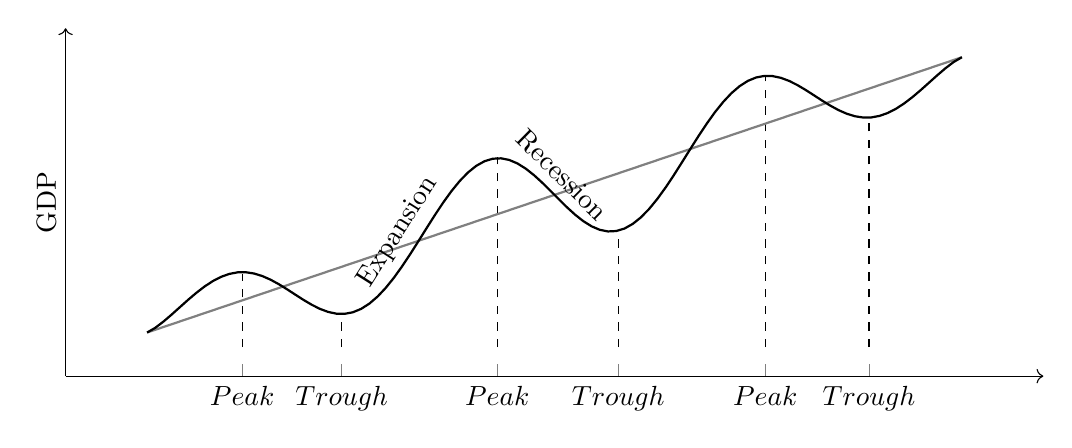
\begin{tikzpicture}
\begin{axis}[
    domain=0:6*pi,
    samples=100,
    axis lines*=left, 
    axis line style={->},
    xtick={2.2, 4.5, 8.1, 10.9, 14.3, 16.7}, ytick=\empty,
    xticklabels = {$Peak$, $Trough$, $Peak$, $Trough$, $Peak$, $Trough$},
    width=14cm, height=6cm,
%    xlabel={time}, 
    ylabel={GDP}
]       
\addplot[mark=none, dashed] coordinates {(2.2, -1) (2.2, 4)};
\addplot[mark=none, dashed] coordinates {(4.5, -1) (4.5, 1)}; 
\addplot[mark=none, dashed] coordinates {(8.1, -1) (8.1, 12)}; 
\addplot[mark=none, dashed] coordinates {(10.9, -1) (10.9, 6.6)}; 
\addplot[mark=none, dashed] coordinates {(14.3, -1) (14.3, 17.5)}; 
\addplot[mark=none, dashed] coordinates {(16.7, -1) (16.7, 14.9)}; 
\addplot [thick, gray] {x};
\addplot [thick, black] {x + 4*sin(deg(x)) * sin(deg(x/6))^0.5}
%    node [pos=0.1, anchor=south] {Peak}
    node [pos=0.3, anchor=south, sloped] {Expansion}
    node [pos=0.49, anchor=south, sloped] {Recession}
% Add line to show end of and ... peak and ... line
;
\end{axis}
\end{tikzpicture}

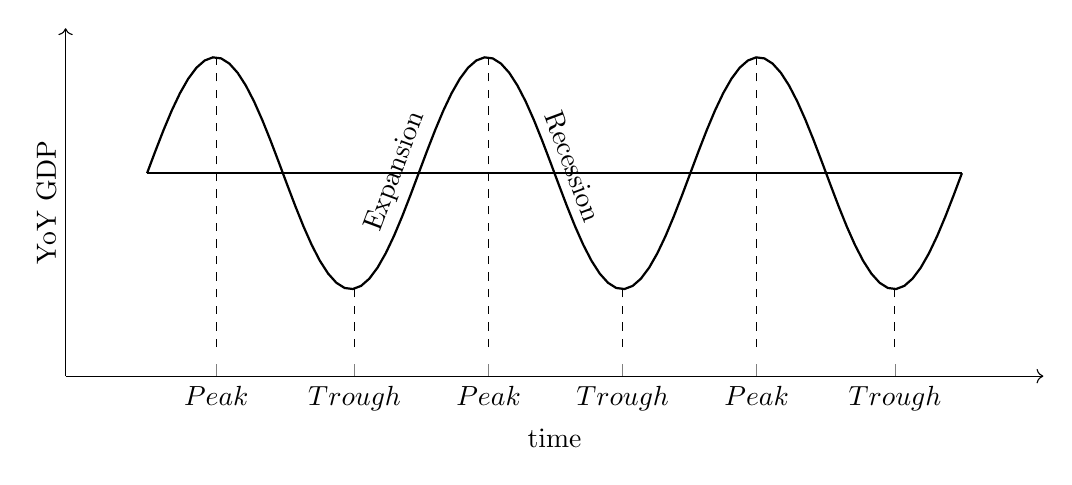
\begin{tikzpicture}
\begin{axis}[
    domain=0:6*pi,
    samples=100,
    axis lines*=left, 
    axis line style={->},
    xtick={1.6, 4.8, 7.9, 11, 14.1, 17.3}, ytick=\empty,
    xticklabels = {$Peak$, $Trough$, $Peak$, $Trough$, $Peak$, $Trough$},
    width=14cm, height=6cm,
    xlabel={time}, 
    ylabel={YoY GDP}
]       
\addplot [thick, black] {sin(deg(x))}
%    node [pos=0.1, anchor=south] {Peak}
    node [pos=0.33, anchor=south, sloped] {Expansion}
    node [pos=0.5, anchor=south, sloped] {Recession}
;
\addplot [thick, black] {0};
\addplot[mark=none, dashed] coordinates {(1.6, -1.5) (1.6, 1)};
\addplot[mark=none, dashed] coordinates {(4.8, -1.5) (4.8, -1)}; 
\addplot[mark=none, dashed] coordinates {(7.9, -1.5) (7.9, 1)}; 
\addplot[mark=none, dashed] coordinates {(11, -1.5) (11,-1)}; 
\addplot[mark=none, dashed] coordinates {(14.1, -1.5) (14.1, 1)}; 
\addplot[mark=none, dashed] coordinates {(17.3, -1.5) (17.3, -1)}; 
\end{axis}
\end{tikzpicture}
    \caption{The Business Cycle theory of GDP and Year on Year GDP}
    \label{fig:Business Cycle}
\end{figure}

\begin{figure}
    \centering
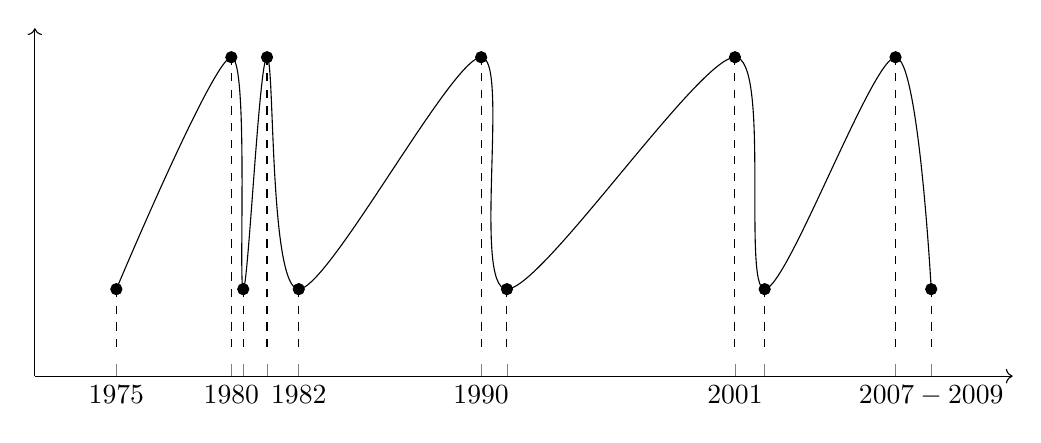
\begin{tikzpicture}
\begin{axis}[
    domain=0:6*pi,
    samples=100,
    axis lines*=left, 
    axis line style={->},
    xtick={2103, 2161, 2167, 2179, 2195, 2287, 2300, 2415,2430, 2496, 2514}, ytick=\empty,
    xticklabels = {$1975$, $1980$,  , , $1982$, $1990$, , $2001$, , ,$2007-2009$},
    width=14cm, height=6cm
%    xlabel={time} 
%    ylabel={YoY GDP}
]       
    \addplot[smooth, mark=*,black] plot coordinates {
	(2103,-1)
    (2161,1)	(2167,-1)
    (2179,1)	(2195,-1)
    (2287,1)	(2300,-1)
    (2415,1)	(2430,-1)
    (2496,1)	(2514,-1)
    };
\addplot[mark=none, dashed] coordinates {(2103, -1.5) (2103, -1)};
\addplot[mark=none, dashed] coordinates {(2161, -1.5) (2161, 1)}; 
\addplot[mark=none, dashed] coordinates {(2167, -1.5) (2167, -1)}; 
\addplot[mark=none, dashed] coordinates {(2179, -1.5) (2179, 1)}; 
\addplot[mark=none, dashed] coordinates {(2195, -1.5) (2195,-1)}; 
\addplot[mark=none, dashed] coordinates {(2287, -1.5) (2287, 1)}; 
\addplot[mark=none, dashed] coordinates {(2300, -1.5) (2300,-1)}; 
\addplot[mark=none, dashed] coordinates {(2415, -1.5) (2415, 1)}; 
\addplot[mark=none, dashed] coordinates {(2430, -1.5) (2430, -1)}; 
\addplot[mark=none, dashed] coordinates {(2496, -1.5) (2496, 1)}; 
\addplot[mark=none, dashed] coordinates {(2514, -1.5) (2514, -1)}; 
\end{axis}
\end{tikzpicture}
    \caption{Business cycles from 1975 to 2009 of the American Economy according to the NBER}
    \label{fig:NBER BS}
\end{figure}




more information can be found in \cite{de_greef_national_2009}


\newpage

\subsection{Questionnaire}
\label{sec:Questionnaire}

\subsection*{General presentation}

Almost the same for everyone, some differences depending on the sector (Industry $\neq$ Services)


Answers are giving by mail, email, on the phone or by fax.


\subsection*{Questions NS975}
Questions taken into account for NS975:
....

originally question Q18, 27, 32 and 33, for simplicity numbered here as 1, 2, 3 and 4.

\subsubsection*{Verloop en beoordeling}
\begin{enumerate}
    \item Uw huidige voorraad van dit product beschouwt u, voor het seizoen, als: \\
	$\Square$	hoger dan normaal (te hoog)	$\Square$	normaal (voldoende)	$\Square$ lager dan normaal (te laag)
	
    \item Uw huidige gezamenlijke orderpositie voor dit product beschouwt u als: \\
	$\Square$ hoger dan normaal $\Square$ normaal $\Square$ lager dan normaal
\end{enumerate}

\subsubsection*{Vooruitzichten voor de volgende drie maanden} 
\begin{enumerate}
\setcounter{enumi}{2}
    \item Het personeel (arbeiders en technici) tewerkgesteld voor de fabricatie van dit product zal volgens u: \\
	$\Square$ worden uitgebreid $\Square$ onveranderd blijven $\Square$ worden verminderd
						
    \item De vraag van uw klanten naar dit product zal volgens u:  \\
	$\Square$ belangrijker $\Square$ even belangrijk $\Square$ minder belangrijk \\	
	zijn dan gewoonlijk tijdens die periode van het jaar.
\end{enumerate}

The first question has to be interpreted the opposite way as of the three other questions. ...


\subsubsection*{Changes over time}

Questionnaire in 1990 (\autoref{Questionnaire1990}) almost same as today


see appendix \autopageref{Questionnaire2018} for the full questionnaire


\subsection{Weighting procedure}
\label{sec:Weighting procedure}

According to the size of the company, measured different ways depending on the sector ........

\subsection{Globalisation procedure}
\label{sec:Globalisation procedure}
Based on the size of the sector in which the company is.
The globalisation procedure got quite complex over time. See the globalisation tree for the Industry survey \autopageref{fig:tree}



\section{Calculation of the Indicator}

This section presents the method for calculating the indicator. 
The calculation in itself is standard, but the different ways to write it are important for interpretation and to better understand the following chapters.

\subsection{Unweighted Indicator}

The calculation of the unweighted indicator for a specific question at a specific time can be written as follow;

\begin{equation}
    E(X) = \frac{ \sum_{i=1}^n x_i}{n}
\end{equation} 
where 

$x_i$ is the answer of the respondent i and can each take value -1, 0 and 1 

$n$ is the total of respondents \\

Since x can only take three different values, we can decompose it into 

\begin{equation}
    E(X) = \frac{ \sum_{i=1}^n x_{+i} + \sum_{i=1}^n x_{Ni} + \sum_{i=1}^n x_{-i}}{n}
\end{equation} 

where 

$x_{+i}$, $x_{Ni}$ and $x_{-i}$ are the positive(+), neutral (N) and negative (-) answers of the respondent i

$n$ is the total of respondents

We know that $\sum_{i=1}^n x_{Ni} = 0$ so we can write

\begin{equation}
    E(X) = \frac{\sum_{i=1}^n x_{+i}}{n}  + \frac{\sum_{i=1}^n x_{-i}}{n}
\end{equation} 

${\sum_{i=1}^n x_{+i}}/{n}$ is the proportion of positive answers and ${\sum_{i=1}^n x_{-i}}/{n}$ is the negative proportion of negative answer so for simplicity we write it 

\begin{equation}
    E(X) = \pi_+ - \pi_-
\end{equation}
where $\pi_+$ and $\pi_-$ are the proportion of respondents answering positive and negative. $\pi$ is use here also in the probabilistic way as it can also be seen as the probability that a respondent answers positive, negative or neutral ($\pi_0$) with $\pi_+ + \pi_0 + \pi_- =1$.



\subsection{Weighted Indicator}

\subsubsection{Globalisation procedure}

\subsubsection{Weighting procedure}

\subsubsection{Calculation}

\begin{equation}
    E(X) = \frac{ \sum_{i=1}^n \left(\omega_i p_i x_i \right)}{\sum_{i=1}^n \omega_i p_i}
\end{equation} 
where \\
$x_i$ is the answer of the respondent i and can each take value -1, 0 and 1 \\
$p_i$ is the weight of the globalisation of the company i \\
$\omega_i$ is the weight of the company i


\begin{equation}
    E(X) = \frac{ \sum_{i=1}^n \omega_{+i} p_{+i} x_{+i} + \sum_{i=1}^n \omega_{Ni} p_{Ni} x_{Ni} + \sum_{i=1}^n \omega_{-i} p_{-i} x_{-i}}{n}
\end{equation} 

\begin{equation}
    E(X) = \frac{ \sum_{i=1}^n \omega_{+i} p_{+i} x_{+i}}{n} + \frac{\sum_{i=1}^n \omega_{-i} p_{-i} x_{-i}}{n}
\end{equation} 


\begin{equation}
    E(X) = \pi_+ - \pi_-
\end{equation}

where $\pi_+$ and $\pi_-$ are the \textbf{weighted} proportion of respondents answering positive and negative. $\pi$ is use here also in the probabilistic way as it can also be seen as the probability that a respondent answers positive, negative or neutral ($\pi_0$) with $\pi_+ + \pi_0 + \pi_- =1$.




\subsection{Properties}

E(X) has -1 as lower bound and 1 as upper bound






\subsection{Take different questions into account}

The previous calculations where specific to each question. The published indicators are usually taking different survey questions into account. For example the Industry indicator that we will be interested in is composed of four questions that have all the same weight:

\begin{equation}
    \mbox{Industry Business Indicator}\ = \frac{E(X_{Q1}) + E(X_{Q2}) + E(X_{Q3}) + E(X_{Q4})}{4}
\end{equation}

where 
$E(X_{Q1})$, $E(X_{Q2})$, $E(X_{Q3})$ and $E(X_{Q4})$ are the different averages for question 18, 27, 32 and 33 (can be weighted or unweighted)

can also been seen as the mean of the answers for each participant at each period then combined together

\begin{equation}
    \mbox{Industry Business Indicator}\ = \frac{\sum_{i=1}^n \left(x_{i Q1} + x_{i Q2} + x_{i Q3} + x_{i Q4} \right) / 4}{n}
\end{equation}


\chapter{The Variance of the Indicator}

The variance is, with the mean, one of the first tool for Statisticians to study a certain variable.

In the context of the Business Survey, the variance haven't been used much.

\subsubsection{The added info of the variance}



\subsubsection{variance as a measure of the dispersion of the responses}

In statistics, the variance has two m

Here we want to know to what extend respondents agree with each others.

\begin{figure}
    \centering
\begin{tikzpicture}
    \begin{axis}[every axis plot post/.append style={
        mark=none,domain=-3:3,samples=50,smooth}, % All plots: from -2:2, 50 samples, smooth, no marks
          axis x line*=bottom, % no box around the plot, only x and y axis
          axis y line*=left, % the * suppresses the arrow tips
          xtick=\empty, ytick=\empty,
          width=10cm, height=4cm,
          enlargelimits=upper] % extend the axes a bit to the right and top
          \addplot {gauss(0,0.5)};
          \addplot {gauss(0,1)};
        %  \addplot [ybar, bar width=5pt] coordinates { (-1, 1) (0, 3)};
    \end{axis}
\end{tikzpicture}
    \caption{The Variance}
    \label{fig:var_explanation}
\end{figure}

\begin{figure}
    \centering
  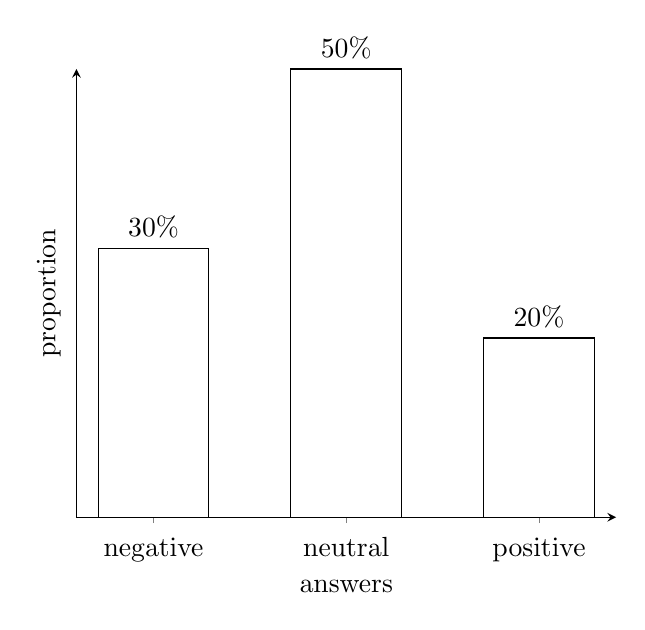
\begin{tikzpicture} %[font=\small]
    \begin{axis}[
      ybar,
      bar width=40pt,
      xlabel={answers},
      ylabel={proportion},
      ymin=0,
      ytick=\empty,
      xtick=data,
      axis x line=bottom,
      axis y line=left,
      enlarge x limits=0.2,
      symbolic x coords={negative,neutral,positive},
      xticklabel style={anchor=base,yshift=-\baselineskip},
      nodes near coords={\pgfmathprintnumber\pgfplotspointmeta\%}
    ]
      \addplot[fill=white] coordinates {
        (negative,30)
        (neutral,50)
        (positive,20)
      };
    \end{axis}
  \end{tikzpicture}
    \caption{Caption}
    \label{fig:hist_example}
\end{figure}




\subsubsection{difference sampling error and variance}

precision

here variance is a measure of the "dispersion" of the answers.

\subsubsection{difference between nominal and continuous variable variance}


As done for the Indicator, two different variances will be take into account here, the weighted and the unweighted variance of the indicator.


\section{Variance of the Unweighted Indicator}

The main variance

cite

\begin{eqnarray}
     \Var(X) &=& E \left[ \left(X-E(X) \right)^2 \right] \nonumber \\ \nonumber \\
     &=& E\left( X^2\right) - E\left( X\right)^2 \nonumber \\ \nonumber \\
     &=& \left( \frac{\sum_{i=1}^n x_{+i}^2}{n} \right) + \left( \frac{\sum_{i=1}^n x_{Ni}^2}{n} \right) + \left( \frac{\sum_{i=1}^n x_{-i}^2}{n} \right) - E(X)^2  \nonumber \\ \nonumber \\
     &=& \pi_+ + \pi_- - ( \pi_+ - \pi_- )^2 \label{var1}
\end{eqnarray}

Since $\left( \frac{\sum_{i=1}^n x_{Ni}^2}{n} \right) = 0$ ,
$x_{+i}^2 = x_{+i}$, $x_{-i}^2 = x_{-i}$
and $E(X) = \pi_+ - \pi_-$


We then have several different ways to write the previous equation;
\begin{eqnarray}
\Var(X) &=& \pi_+ + \pi_- - ( \pi_+ - \pi_- )^2 \nonumber \\
	&=& \pi_+ + \pi_- - E ( X )^2 \label{var2} \\
	&=& 1 - \pi_n - E(X)^2 \label{var3}
\end{eqnarray}

\autoref{var1} is interesting 

Equation \ref{var2}

Equation \ref{var3}




\section{Variance of the Weighted Indicator}

\begin{equation}
\Var(X) = \frac{1}{\sum \omega_i p_i } \sum^N _{i=1} \omega_i p_i (X_i - \bar{X})^2
\end{equation}

\begin{eqnarray}
\Var(X) &=& \pi_+ + \pi_- - ( \pi_+ - \pi_- )^2 \\
	&=& \pi_+ + \pi_- - E ( X )^2 \\
	&=& 1 - \pi_0 - E(X)^2
\end{eqnarray}


\subsection{Properties}

\begin{figure}[h]
    \centering
    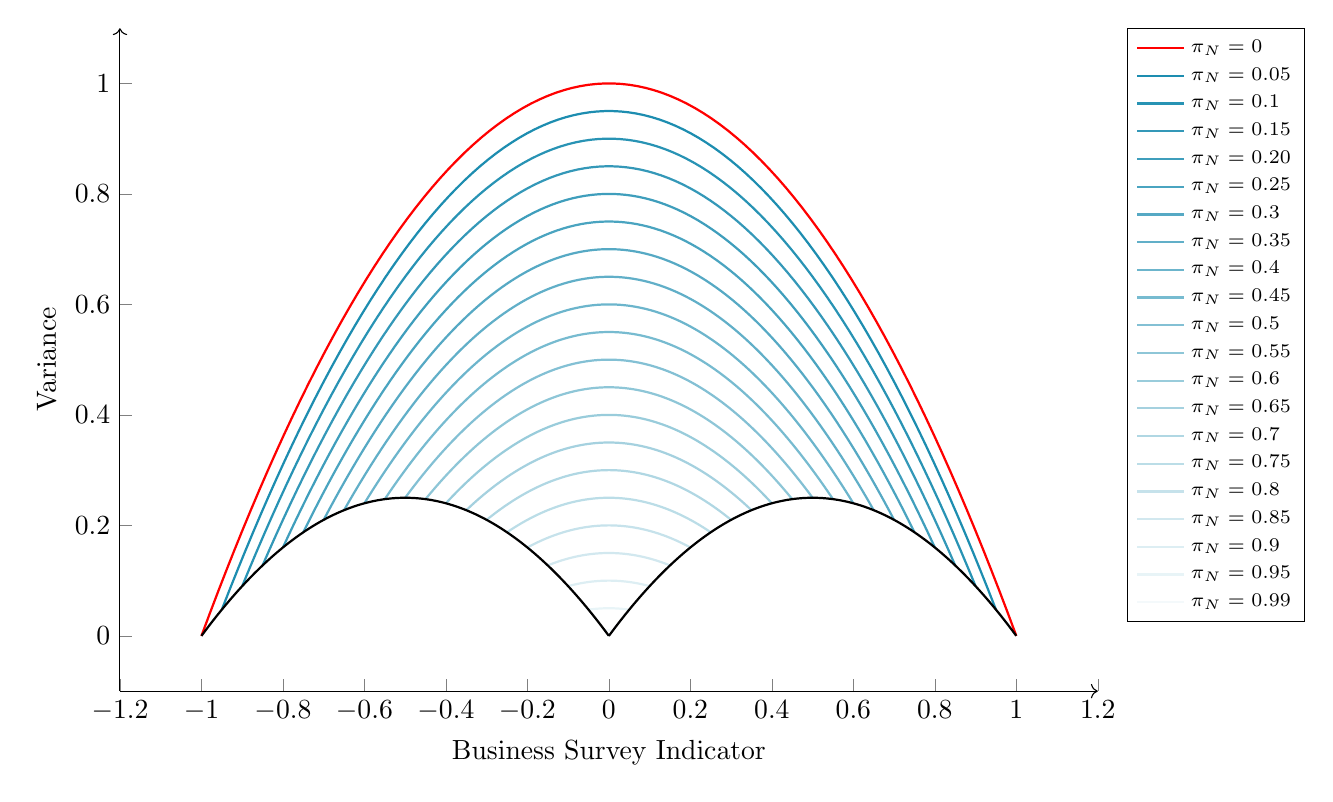
\begin{tikzpicture}
    \tikzset{
      legendmatrix/.style={% style for legends
        draw,% draw a border for the legend
        outer sep=.3333em,% additional space to the axis label
        nodes={rotate=90,anchor=base west,outer sep=0pt},% rotate the nodes inside the matrix
        /pgfplots/every crossref picture/.append style={yshift=.75ex}% rotate the legend images
      }
    }
    \begin{axis}[
        domain=-1:1,
        samples=100,
        axis lines*=left, 
        axis line style={->},
        width=14cm, height=10cm,
        xlabel={Business Survey Indicator}, ylabel={Variance},
    legend pos= outer north east, legend cell align=left,
     legend style={font=\scriptsize}
     ]       
    \addplot [thick, red, domain = -1:1] {1 - x^2};
    \addplot [thick, bluetitle!100, domain = -0.95:0.95] {1 - 0.05 - x^2};
    \addplot [thick, bluetitle!95, domain = -0.9:0.9] {1 - 0.1 - x^2};
    \addplot [thick, bluetitle!90, domain = -0.85:0.85] {1 - 0.15 - x^2};
    \addplot [thick, bluetitle!85, domain = -0.8:0.8] {1 - 0.2 - x^2};
    \addplot [thick, bluetitle!80, domain = -0.75:0.75] {1 - 0.25 - x^2};
    \addplot [thick, bluetitle!75, domain = -0.7:0.7] {1 - 0.3 - x^2};
    \addplot [thick, bluetitle!70, domain = -0.65:0.65] {1 - 0.35 - x^2};
    \addplot [thick, bluetitle!65, domain = -0.6:0.6] {1 - 0.4 - x^2};
    \addplot [thick, bluetitle!60, domain = -0.55:0.55] {1 - 0.45 - x^2};
    \addplot [thick, bluetitle!55, domain = -0.5:0.5] {1 - 0.5 - x^2};
    \addplot [thick, bluetitle!50, domain = -0.45:0.45] {1 - 0.55 - x^2};
    \addplot [thick, bluetitle!45, domain = -0.4:0.4] {1 - 0.6 - x^2};
    \addplot [thick, bluetitle!40, domain = -0.35:0.35] {1 - 0.65 - x^2};
    \addplot [thick, bluetitle!35, domain = -0.3:0.3] {1 - 0.7 - x^2};
    \addplot [thick, bluetitle!30, domain = -0.25:0.25] {1 - 0.75 - x^2};
    \addplot [thick, bluetitle!25, domain = -0.2:0.2] {1 - 0.8 - x^2};
    \addplot [thick, bluetitle!20, domain = -0.15:0.15] {1 - 0.85 - x^2};
    \addplot [thick, bluetitle!15, domain = -0.1:0.1] {1 - 0.9 - x^2};
    \addplot [thick, bluetitle!10, domain = -0.05:0.05] {1 - 0.95 - x^2};
    \addplot [thick, bluetitle!05, domain = -0.01:0.01] {1 - 0.99 - x^2};
 %    \addplot [thick, black, domain = -1:0] { - ((x+0.5)^2) + 0.25};
 %    \addplot [thick, black, domain = 0:1] { - ((x-0.5)^2) + 0.25};
     \addplot [thick, black, domain = -1:0] {-x-x^2};
     \addplot [thick, black, domain = 0:1] {x-x^2};
%     \addplot [thick, black, domain = -1:1] {(x^2)*(-y)-(y^2)/2 + y};    
	\addlegendentry{$\pi_N = 0$}
    \addlegendentry{$\pi_N = 0.05$}
    \addlegendentry{$\pi_N = 0.1$}
    \addlegendentry{$\pi_N = 0.15$}
    \addlegendentry{$\pi_N = 0.20$}
    \addlegendentry{$\pi_N = 0.25$}
    \addlegendentry{$\pi_N = 0.3$}
    \addlegendentry{$\pi_N = 0.35$}
    \addlegendentry{$\pi_N = 0.4$}
    \addlegendentry{$\pi_N = 0.45$}
    \addlegendentry{$\pi_N = 0.5$}
    \addlegendentry{$\pi_N = 0.55$}
    \addlegendentry{$\pi_N = 0.6$}
    \addlegendentry{$\pi_N = 0.65$}
    \addlegendentry{$\pi_N = 0.7$}
    \addlegendentry{$\pi_N = 0.75$}
    \addlegendentry{$\pi_N = 0.8$}
    \addlegendentry{$\pi_N = 0.85$}
    \addlegendentry{$\pi_N = 0.9$}
    \addlegendentry{$\pi_N = 0.95$}
    \addlegendentry{$\pi_N = 0.99$}
    \end{axis}
    \end{tikzpicture}
    \caption{Plot of the BSI on it's variance for different values of $\pi_N$ ($\pi_N = 1 - \pi_+ - \pi_-$)}
    \label{fig:var properties}
\end{figure}






\subsubsection{Property 1: The variance of X is bounded between -1 and 1}

\subsubsection{Property 2: The variance = A5 and E(X)}


\subsubsection{Property 3: .....}

upper bound : 
\begin{equation}
    \Var(X) = 1 - 0 - \E(X)^2
\end{equation}

lower bound : 
\begin{eqnarray}
\Var(X) &=& - (\E(X) + 0,5)^2 + 0,25 \quad \text{where } \Var(X) \text{ is between -1 and 0} \\
    &=& X - X^2 
\end{eqnarray}

\begin{eqnarray}
    \Var(X) &=& - (\E(X) - 0,5)^2 + 0,25 \quad \text{where } \Var(X) \text{ is between 0 and 1} \\
        &=& - X - X^2
\end{eqnarray}
    

\section{Take different questions into account}

Since 

\begin{eqnarray}
    \Var \left(\frac{X_{Q1} + X_{Q2} + X_{Q3} + X_{Q4}}{4} \right) &\neq&
    \frac{\Var(X_{Q1}) + \Var(X_{Q2}) + \Var(X_{Q3}) + \Var(X_{Q4})}{16} \nonumber
\end{eqnarray}


\begin{eqnarray}
    \Var \left(\frac{X+Y}{2} \right) = \frac{1}{4} \left( \Var (X) + \Var(Y) + \Cov (X,Y) \right) 
\end{eqnarray}

\begin{eqnarray}
    \Var \left(\frac{X_{Q1} + X_{Q2} + X_{Q3} + X_{Q4}}{4} \right) &=& \frac{1}{16} \large[ \Var(X_{Q1}) + \Var(X_{Q2}) + \Var(X_{Q3}) + \Var(X_{Q4}) \nonumber \\
    && + \Cov (X_{Q1},X_{Q2}) + \Cov (X_{Q1},X_{Q3}) + \Cov (X_{Q1},X_{Q4}) \nonumber \\
    &&  + \Cov (X_{Q2},X_{Q3}) + \Cov (X_{Q2},X_{Q4}) + \Cov (X_{Q3},X_{Q4}) \large] \nonumber
\end{eqnarray}

\begin{eqnarray}
    \Var \left(\frac{X_{Q1} + X_{Q2} + X_{Q3} + X_{Q4}}{4} \right) 
    &=& \Var \left(\frac{\sum_{i=1}^n \left(x_{i Q1} + x_{i Q2} + x_{i Q3} + x_{i Q4} \right)}{4n} \right) \nonumber \\
    &=& \Var \left(\frac{\pi_{1+} + \pi_{2+} + \pi_{3+} + \pi_{4+} - \pi_{1-} - \pi_{2-} - \pi_{3-} - \pi_{4-} }{4} \right) \nonumber \\
    &=& \frac{1}{16} \Var \left(\pi_{1+} + \pi_{2+} + \pi_{3+} + \pi_{4+} - \pi_{1-} - \pi_{2-} - \pi_{3-} - \pi_{4-} \right) \nonumber \\
\end{eqnarray}

\begin{eqnarray}
    \Var \left(\frac{X_{Q1} + X_{Q2} + \ldots + X_{Qn}}{n} \right) 
    &=& \Var \left(\frac{\pi_{1+} + \pi_{2+} + \ldots + \pi_{n+} - \pi_{1-} - \pi_{2-} - \ldots - \pi_{n-} }{n} \right) \nonumber \\
    &=& \frac{1}{n^2} \Var \left(\pi_{1+} + \pi_{2+} + \ldots + \pi_{n+} - \pi_{1-} - \pi_{2-} - \ldots - \pi_{n-} \right) \nonumber \\
\end{eqnarray}


\newpage

\section{Discussion regarding the 'true variance'}

There is another way to calculate the variance that have been ignored for, that is calculating the variance for each lowest group of globalisation, and then combine those calculated variances.


Interestingly, it have been calculated for several Questions of the business barometer, and it is approximately 10 times smaller than the variance based on all the answer a ones.



The reasons why it will not be used here
- losing information
- weight of globalisation taken into account in the weighted variance




\chapter{The Indicator of the Evolution of Individual Responses}

 \subsubsection{Why this new indicator}

Also Called Z indicator

Can be better understood as the indicator of the Changes in individual answers between t-1 and t

cite the paper by INSEE % \cite{}


 An issue for this indicator was to find an optimal name for it so that it would be easily understand by the largest number.
 
 

\subsubsection{The Indicator of the Evolution of Individual Responses}


\subsubsection{Explain the new indicator}

\begin{center}
\begin{tabular}{r | r | c c c | }
\multicolumn{1}{r}{} & \multicolumn{1}{r}{} &	\multicolumn{3}{c}{$t$} \\ \cline{3-5}
\multicolumn{1}{r}{} & 		& \textbf{-} & \textbf{0} & \textbf{+} \\ \cline{2-5}
		&    \textbf{-} & $\pi_{--}$	& $\pi_{-0}$	& $\pi_{-+}$ \\ 
$t-1$ & \textbf{0} & $\pi_{0-}$	& $\pi_{00}$	& $\pi_{0+}$	\\
		&    \textbf{+} & $\pi_{+-}$	& $\pi_{+0}$	& $\pi_{++}$ \\ \cline{2-5}
\end{tabular}    
\end{center}

where

\begin{equation}
\pi_{++} + \pi_{+0} + \pi_{+-} + \pi_{0+} + \pi_{00} + \pi_{0-} + \pi_{-+} + \pi_{-0} + \pi_{--} = 1
\end{equation}

The Indicator of the evolution of the individual responses can be obtained by

\begin{equation}
E(Z) = \pi_{0+} + \pi_{-0} - \pi_{+0} - \pi_{0-} +2\pi_{-+} -2\pi_{+-} 
\end{equation}

where
$\pi$ is the proportion/probability of respondent answering (-,0,+) at $t-1$ and $t$ 


\begin{equation}
E(Z) = \pi_{0+} + \pi_{-0} - \pi_{+0} - \pi_{0-} +2\pi_{-+} -2\pi_{+-} = 
\begin{tabular}{r|r r r}
    			& \textbf{-} & \textbf{0} & \textbf{+} \\\hline
    \textbf{-} 	& 0		& +1	& +2	\\
    \textbf{0} 	& -1	& 0		& +1	\\
    \textbf{+} 	& -2	& -1	& 0		\\
\end{tabular}
\end{equation}

\subsubsection{Interpretation}



\section{Generalisation for n time frames}

Changes in the economy are usually taking several months to 

Therefor it's interesting to take a larger period into account.

There are mainly to ways to generalise this method. \\ A simple generalisation is to use t-n rather than t-1. You compare then that period t-n with the the answer at t, without taking the between answers into account.

Another generalisation is as follow


\subsection{Take the evolution from t-n to t}

To keep it simple, rather than comparing the answers at t with t-1, we can also look at t vs t-2 and so on







\chapter{The Variance of the Evolution of Individual Responses (Volatility of Responses)} \label{Chapter:Z}

That we will also call the \textbf{volatility of the indicator}, in the sens that the variance of the evolution of the indicator account for the dispersion of the difference in answers over a two times period.

In this case, the highers variance of Z, will be obtained when half of the companies went from a negative answer to a positive answer and the other half did the opposite and changed from a positive answer at t-1 to a negative answer at t. 

waza see Chapter \ref{Chapter:Z}

The idea is that this variance of Z is complementary to the estimation of Z since they have two very interesting but different interpretations.
Further interpretation will be 

\section{Presentation}



\begin{equation}
\pi_{++} + \pi_{+0} + \pi_{+-} + \pi_{0+} + \pi_{00} + \pi_{0-} + \pi_{-+} + \pi_{-0} + \pi_{--} = 1 
\end{equation}

\begin{eqnarray}
Var(Z) &=& \pi_{0+} + \pi_{-0} + \pi_{+0} + \pi_{0-} +4\pi_{-+} +4\pi_{+-} \nonumber \nonumber \\ 
&&	- (\pi_{0+} + \pi_{-0} - \pi_{+0} - \pi_{0-} +2\pi_{-+} -2\pi_{+-})^2 \nonumber \\
&=& \pi_{0+} + \pi_{-0} + \pi_{+0} + \pi_{0-} +4\pi_{-+} +4\pi_{+-} - E(Z)^2 \nonumber \\
&=& 1 - \pi_{++} - \pi_{00} - \pi_{--} + 3\pi_{+-} + 3\pi_{-+} - E(Z)^2
\end{eqnarray}

\begin{eqnarray*}
Var(Z) &=& 
\left(\begin{tabular}{r|r r r}
    			& \textbf{-} & \textbf{0} & \textbf{+} \\\hline
    \textbf{-} 	& 0		& +1	& +4	\\
    \textbf{0} 	& +1	& 0		& +1	\\
    \textbf{+} 	& +4	& +1	& 0		\\
\end{tabular} \right)
- \left(
\begin{tabular}{r|r r r}
    			& \textbf{-} & \textbf{0} & \textbf{+} \\\hline
    \textbf{-} 	& 0		& +1	& +2	\\
    \textbf{0} 	& -1	& 0		& +1	\\
    \textbf{+} 	& -2	& -1	& 0		\\
\end{tabular}
\right)^2  \\
&=& \left( \begin{tabular}{r|r r r}
    			& \textbf{-} & \textbf{0} & \textbf{+} \\\hline
    \textbf{-} 	& 0		& +1	& +4	\\
    \textbf{0} 	& +1	& 0		& +1	\\
    \textbf{+} 	& +4	& +1	& 0		\\
\end{tabular} \right)
- \left(E(Z)\right)^2 	\\
&=& 1 +  \left(\begin{tabular}{r|r r r}
    			& \textbf{-} & \textbf{0} & \textbf{+} \\\hline
    \textbf{-} 	& -1	& 0		& +3	\\
    \textbf{0} 	& 0		& -1	& 0	\\
    \textbf{+} 	& +3	& 0		& -1		\\
\end{tabular} \right)
 - \left(E(Z)\right)^2	\\
\end{eqnarray*}



\subsection{Properties}

\subsubsection{Property 1: the variance of Z is bounded between -1 and 1}


\subsubsection{Property 2: }






\chapter{Non-Response, Dropout, Attrition and Seasonal Effects}

\begin{table}[!htbp] \centering 
  \caption{Correlation Between Time and different variables} 
  \label{} 
\begin{tabular}{@{\extracolsep{5pt}} cccccccc} 
\\[-1.8ex]\hline 
\hline \\[-1.8ex] 
  & GDP & YoY GDP & BSI & Var & Z\_I & Var\_Z\_I \\ 
\hline \\[-1.8ex] 
Time & $-0.223$ & $-0.352$ & $0.148$ & $-0.775$ & $0.060$ & $-0.728$ \\ 
\hline \\[-1.8ex] 
\end{tabular} 
\end{table}


\begin{figure}[H]
    \centering
    \captionsetup{justification=centering}
    \includegraphics[scale=0.5]{Graphs/plot_var.pdf}
    \caption{Plot }
    \label{XXXX}
\end{figure}


\section{Non-Response}

plot non-response


\newpage
\section{Dropout}

Non parametric test \cite{das_nonparametric_2011}


\newpage
\section{Attrition}
Attrition / Panel Conditioning 
Master Thesis done about the Belgian Labor Force Survey, where  attrition was studied \cite{priyana_hardjawidjaksana_investigating_2019}

Non parametric test \cite{das_nonparametric_2011}


limitation: only some periods of 


\newpage
\section{Seasonal Effects}
The National Bank, before publishing the Business Survey Indicator, applies a X11 seasonal correction

The literature about seasonal effects is very rich and variate

- NBB developed JDemetra+ and has since been recommended by the ECB and Eurostat for all NSI in Europe.


at the same time the department of Business Survey uses as a X11 adapted method to correct for seasonality because don't want to correct for previous publications.


Methodology \\
- test for seasonality \\
- run the analysis without corrections \\
- apply corrections and see if more accurate \\

\subsection*{Seasonal correction of the Indicator}

\subsection*{Seasonal correction of the Variance}

\subsection*{Seasonal correction of the Indicator of the Evolution}

\subsection*{Seasonal correction of the Variance of Z}

\subsection*{Seasonal correction of the Proportions}

\section{Limitations}
 ?? 
 
explain the issue of seasonal correction on "future data" 



\chapter{Exploratory Analysis}


\section{Data At hand}

Four questions

1988 - 2018

\section{Small vs Large}


\section{By Sector}

\section{Correlations}

There are three different correlations that need to be looked at

\section{Correlation between questions}

\begin{table}[!htbp] \centering 
  \caption{Correlation Matrix} 
  \label{} 
\begin{tabular}{@{\extracolsep{5pt}} ccccc} 
\\[-1.8ex]\hline 
\hline \\[-1.8ex] 
 & E\_1 & E\_2 & E\_3 & E\_4 \\ 
\hline \\[-1.8ex] 
E\_1 & $1$ & $0.262$ & $0.412$ & $0.416$ \\ 
E\_2 & $0.262$ & $1$ & $0.939$ & $0.876$ \\ 
E\_3 & $0.412$ & $0.939$ & $1$ & $0.938$ \\ 
E\_4 & $0.416$ & $0.876$ & $0.938$ & $1$ \\ 
\hline \\[-1.8ex] 
\end{tabular} 
\end{table}
 
\newpage
\section{Auto-Correlation}

\begin{figure}[H]
    \centering
    \captionsetup{justification=centering}
    \includegraphics[scale=0.5]{Graphs/ACF.pdf}
    \caption{Plot }
    \label{ACF}
\end{figure}

\begin{figure}[H]
    \centering
    \captionsetup{justification=centering}
    \includegraphics[scale=0.45]{Graphs/ACF_GDP.pdf}
    \caption{Plot }
    \label{ACF_GDP}
\end{figure}



\section{Correlation with GDP}

Belgian industry claims 25\% of the labour force in Belgium and have been shown as been the best indicator to predict the year to year GDP
cite{Alain Quartier and Isabelle}


\subsection*{GDP vs GDP YoY}


\subsection*{Correlation}

\begin{table}[!htbp] \centering 
  \caption{Correlation Matrix} 
  \label{} 
\begin{tabular}{@{\extracolsep{5pt}} cccccccc} 
\\[-1.8ex]\hline 
\hline \\[-1.8ex] 
 & GDP & GDP\_year & E\_I & E\_1 & E\_2 & E\_3 & E\_4 \\ 
\hline \\[-1.8ex] 
GDP & $1$ & $0.628$ & $0.502$ & $0.222$ & $0.439$ & $0.473$ & $0.556$ \\ 
GDP\_year & $0.628$ & $1$ & $0.707$ & $0.092$ & $0.729$ & $0.703$ & $0.717$ \\ 
E\_I & $0.502$ & $0.707$ & $1$ & $0.483$ & $0.952$ & $0.982$ & $0.963$ \\ 
E\_1 & $0.222$ & $0.092$ & $0.483$ & $1$ & $0.266$ & $0.414$ & $0.406$ \\ 
E\_2 & $0.439$ & $0.729$ & $0.952$ & $0.266$ & $1$ & $0.942$ & $0.886$ \\ 
E\_3 & $0.473$ & $0.703$ & $0.982$ & $0.414$ & $0.942$ & $1$ & $0.938$ \\ 
E\_4 & $0.556$ & $0.717$ & $0.963$ & $0.406$ & $0.886$ & $0.938$ & $1$ \\ 
%\vdots & \vdots & \vdots & \vdots & \vdots & \vdots & \vdots \\
\hline \\[-1.8ex] 
\end{tabular} 
\end{table} 

\begin{figure}[H]
    \centering
    \includegraphics[scale=0.5]{Graphs/ggpairs.pdf}
    \caption{Plot }
    \label{ggpairs}
\end{figure}


\section{GDP vs Explanatory Indicators}

\begin{table}[H] \centering 
  \caption{Correlation Matrix} 
  \label{} 
\begin{tabular}{@{\extracolsep{5pt}} ccccccc} 
\\[-1.8ex]\hline 
\hline \\[-1.8ex] 
 & GDP & GDP\_year & E\_I & Var\_I & Z\_I & Var\_Z\_I \\ 
\hline \\[-1.8ex] 
GDP & $1$ & $0.628$ & $0.502$ & $-0.074$ & $0.151$ & $0.021$ \\ 
GDP\_year & $0.628$ & $1$ & $0.707$ & $-0.101$ & $-0.058$ & $0.011$ \\ 
E\_I & $0.502$ & $0.707$ & $1$ & $-0.615$ & $0.166$ & $-0.484$ \\ 
Var\_I & $-0.074$ & $-0.101$ & $-0.615$ & $1$ & $-0.045$ & $0.887$ \\ 
Z\_I & $0.151$ & $-0.058$ & $0.166$ & $-0.045$ & $1$ & $-0.072$ \\ 
Var\_Z\_I & $0.021$ & $0.011$ & $-0.484$ & $0.887$ & $-0.072$ & $1$ \\ 
\hline \\[-1.8ex] 
\end{tabular} 
\end{table} 

\begin{figure}[H]
    \centering
    \includegraphics[scale=0.5]{Graphs/ggpairs2.pdf}
    \caption{Plot }
    \label{ggpairs2}
\end{figure}

\subsection*{GDP vs Indicator}

\subsection*{GDP vs Var}

\subsection*{GDP vs Z}

\subsection*{GDP vs Var Z}


\newpage

\section{Specificity of question 3 and 4, are peoples predictions correct ?}

\begin{table}[!htbp] \centering 
  \caption{Correlation Matrix} 
  \label{} 
\begin{tabular}{@{\extracolsep{5pt}} cccccccc} 
\\[-1.8ex]\hline 
\hline \\[-1.8ex] 
 & GDP & GDP\_year & E\_3 & E\_3\_lag1 & E\_3\_lag2 & E\_3\_lag3 & E\_3\_lag4 \\ 
\hline \\[-1.8ex] 
GDP & $1$ & $0.628$ & $0.477$ & $0.520$ & $0.545$ & $0.546$ & $0.531$ \\
GDP\_year & $0.628$ & $1$ & $0.707$ & $0.679$ & $0.673$ & $0.628$ & $0.560$ \\
E\_3 & $0.477$ & $0.707$ & $1$ & $0.969$ & $0.948$ & $0.906$ & $0.846$ \\
E\_3\_lag1 & $0.520$ & $0.679$ & $0.969$ & $1$ & $0.975$ & $0.940$ & $0.892$ \\
E\_3\_lag2 & $0.545$ & $0.673$ & $0.948$ & $0.975$ & $1$ & $0.974$ & $0.933$ \\
E\_3\_lag3 & $0.546$ & $0.628$ & $0.906$ & $0.940$ & $0.974$ & $1$ & $0.969$ \\
E\_3\_lag4 & $0.531$ & $0.560$ & $0.846$ & $0.892$ & $0.933$ & $0.969$ & $1$ \\ 
\hline \\[-1.8ex] 
\end{tabular} 
\end{table} 


\begin{table}[!htbp] \centering 
  \caption{Correlation Matrix} 
  \label{} 
\begin{tabular}{@{\extracolsep{5pt}} cccccccc} 
\\[-1.8ex]\hline 
\hline \\[-1.8ex] 
 & GDP & GDP\_year & E\_4 & E\_4\_lag1 & E\_4\_lag2 & E\_4\_lag3 & E\_4\_lag4 \\ 
\hline \\[-1.8ex] 
GDP & $1$ & $0.628$ & $0.558$ & $0.555$ & $0.591$ & $0.566$ & $0.536$ \\ 
GDP\_year & $0.628$ & $1$ & $0.719$ & $0.650$ & $0.647$ & $0.593$ & $0.501$ \\ 
E\_4 & $0.558$ & $0.719$ & $1$ & $0.959$ & $0.941$ & $0.890$ & $0.804$ \\ 
E\_4\_lag1 & $0.555$ & $0.650$ & $0.959$ & $1$ & $0.970$ & $0.928$ & $0.863$ \\
E\_4\_lag2 & $0.591$ & $0.647$ & $0.941$ & $0.970$ & $1$ & $0.970$ & $0.917$ \\
E\_4\_lag3 & $0.566$ & $0.593$ & $0.890$ & $0.928$ & $0.970$ & $1$ & $0.959$ \\
E\_4\_lag4 & $0.536$ & $0.501$ & $0.804$ & $0.863$ & $0.917$ & $0.959$ & $1$ \\
\hline \\[-1.8ex] 
\end{tabular} 
\end{table} 





\chapter{Linear (Auto-Regressive) Models}


\section{Method}

\subsection{Month vs Quarterly data}

Error to aggregate everything to quarterly - lost of information

\subsection{Timing of the Data}


The quaterly GDP and the Quaterly YoY GDP is set at t. This is the common way to go..


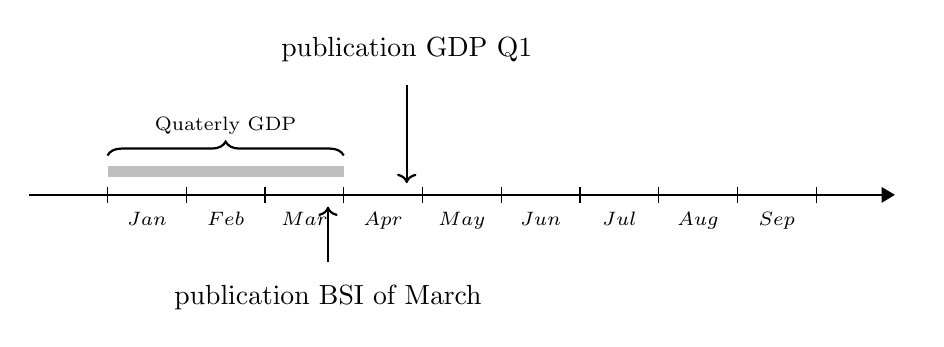
\begin{tikzpicture}
% draw horizontal line   
\draw[thick, -Triangle] (0,0) -- (\ImageWidth,0) node[font=\scriptsize,below left=3pt and -8pt]{ };

% draw vertical lines
\foreach \x in {1,...,10}
\draw (\x cm,3pt) -- (\x cm,-3pt);

\foreach \x/\descr in {1.5/Jan, 2.5/Feb, 3.5/Mar, 4.5/Apr, 5.5/May, 6.5/Jun, 7.5/Jul, 8.5/Aug,9.5/Sep}
\node[font=\scriptsize, text height=1.75ex,
text depth=.5ex] at (\x,-.3) {$\descr$};

% colored bar up
\foreach \x/\perccol in
{1/100,2/75,3/25}
\draw[lightgray, line width=4pt] 
(\x,.3) -- +(1,0);

% braces
\draw [thick ,decorate,decoration={brace,amplitude=5pt}] (1,0.5)  -- +(3,0) 
       node [black,midway,above=4pt, font=\scriptsize] {Quaterly GDP};
%\draw [thick,decorate,decoration={brace,amplitude=5pt}] (6,-.9) -- +(-1,0)
%       node [black,midway,font=\scriptsize, below=4pt] {Publication};

% time of publication
\node[align=center] at (4.8,1.85) {publication GDP Q1};
\draw [thick,->] (4.8,1.4) -- (4.8,0.15);
\node[align=center] at (3.8,-1.3) {publication BSI of March};
\draw [thick,->] (3.8,-0.85) -- (3.8,-0.15);
\end{tikzpicture}

\section{Linear Model}
\begin{eqnarray}
    GDP_{t} = \mu + \sum^n_{i = 1} \sum^q_{j = 0}
       \beta_{1,j} X_{i,t-j} + \epsilon_t 
\end{eqnarray}

Auto-Regressive model
\begin{eqnarray}
    GDP_{t} = \mu + \sum^p_{j = 1} \phi_j GDP_{t-j} +         \sum^n_{i = 1} \sum^q_{j = 0}
       \beta_{1,j} X_{i,t-j} + \epsilon_t 
\end{eqnarray}

where   \\
\begin{tabular}{l l}
    $GDP_t$     & GDP growth over the last semester \\
    $X_{i,t}$   & monthly predictors \\
    $\mu$       & constant \\
    $\phi_j$    & auto-regressive coefficients \\
    $\beta_{i,j}$ & regression coefficients \\
\end{tabular}



\section{Model}

\newpage

\begin{table}[!htbp] \centering 
%  \caption{} 
  \label{} 
\begin{tabular}{@{\extracolsep{5pt}}lD{.}{.}{-3} D{.}{.}{-3} D{.}{.}{-3} D{.}{.}{-3} } 
\\[-1.8ex]\hline 
\hline \\[-1.8ex] 
 & \multicolumn{4}{c}{Linear Regression} \\ 
\cline{2-5} 
\\[-1.8ex] & \multicolumn{4}{c}{Year on Year GDP (in \%)} \\ 
\\[-1.8ex] & \multicolumn{1}{c}{(1)} & \multicolumn{1}{c}{(2)} & \multicolumn{1}{c}{(3)} & \multicolumn{1}{c}{(4)}\\ 
\hline \\[-1.8ex] 
 Constant & 3.434^{***} & 1.114^{***} & -1.829^{**} & -4.052^{***} \\ 
  & (0.170) & (0.255) & (0.867) & (0.922) \\ 
  & & & & \\ 
 3 months lag of YoY GDP &  & 0.690^{***} & 0.525^{***} &  \\ 
  &  & (0.066) & (0.078) &  \\ 
  & & & & \\ 
 BSI & 15.053^{***} & 4.957^{***} & 10.621^{***} & 22.080^{***} \\ 
  & (1.364) & (1.387) & (2.079) & (1.392) \\ 
  & & & & \\ 
 Variance &  &  & 12.831^{***} & 27.506^{***} \\ 
  &  &  & (3.628) & (3.349) \\ 
  & & & & \\ 
\hline \\[-1.8ex] 
Observations & \multicolumn{1}{c}{124} & \multicolumn{1}{c}{123} & \multicolumn{1}{c}{123} & \multicolumn{1}{c}{124} \\ 
R$^{2}$ & \multicolumn{1}{c}{0.499} & \multicolumn{1}{c}{0.743} & \multicolumn{1}{c}{0.767} & \multicolumn{1}{c}{0.679} \\ 
Adjusted R$^{2}$ & \multicolumn{1}{c}{0.495} & \multicolumn{1}{c}{0.738} & \multicolumn{1}{c}{0.761} & \multicolumn{1}{c}{0.673} \\ 
Residual Std. Error & \multicolumn{1}{c}{1.172} & \multicolumn{1}{c}{0.847} & \multicolumn{1}{c}{0.809} & \multicolumn{1}{c}{0.943} \\ 
F Statistic & \multicolumn{1}{c}{121.753$^{***}$} & \multicolumn{1}{c}{173.266$^{***}$} & \multicolumn{1}{c}{130.755$^{***}$} & \multicolumn{1}{c}{127.781$^{***}$} \\ 
\end{tabular} 
\end{table}

\begin{figure}[H]
    \centering
    \captionsetup{justification=centering}
    \includegraphics[scale=0.5]{Graphs/pred1.pdf}
    \caption{Plot }
    \label{pred1}
\end{figure}



\begin{table}[H] \centering 
%  \caption{} 
  \label{} 
\begin{tabular}{@{\extracolsep{5pt}}lD{.}{.}{-3} D{.}{.}{-3} D{.}{.}{-3} D{.}{.}{-3} } 
\\[-1.8ex] & \multicolumn{4}{c}{GDP\_year} \\ 
\\[-1.8ex] & \multicolumn{1}{c}{(1)} & \multicolumn{1}{c}{(2)} & \multicolumn{1}{c}{(3)} & \multicolumn{1}{c}{(4)}\\ 
\hline \\[-1.8ex] 
 Constant & 3.364^{***} & -4.052^{***} & -3.993^{***} & -0.985 \\ 
  & (0.173) & (0.922) & (0.917) & (0.797) \\ 
  & & & & \\ 
 E\_I & 14.491^{***} & 22.080^{***} & 21.579^{***} & 5.629^{***} \\ 
  & (1.390) & (1.392) & (1.421) & (2.091) \\ 
  & & & & \\ 
 E\_I\_diff & 11.538^{*} &  & 8.181 & 24.063^{***} \\ 
  & (6.560) &  & (5.309) & (4.488) \\ 
  & & & & \\ 
 Var\_I &  & 27.506^{***} & 27.105^{***} & 7.179^{**} \\ 
  &  & (3.349) & (3.340) & (3.433) \\ 
  & & & & \\ 
 GDP\_year\_lag1 &  &  &  & 0.687^{***} \\ 
  &  &  &  & (0.076) \\ 
  & & & & \\ 
\hline \\[-1.8ex] 
R$^{2}$ & \multicolumn{1}{c}{0.512} & \multicolumn{1}{c}{0.679} & \multicolumn{1}{c}{0.685} & \multicolumn{1}{c}{0.813} \\ 
Adjusted R$^{2}$ & \multicolumn{1}{c}{0.504} & \multicolumn{1}{c}{0.673} & \multicolumn{1}{c}{0.677} & \multicolumn{1}{c}{0.806} \\ 
Residual Std. Error & \multicolumn{1}{c}{1.162} & \multicolumn{1}{c}{0.943} & \multicolumn{1}{c}{0.938} & \multicolumn{1}{c}{0.729} \\ 
F Statistic & \multicolumn{1}{c}{63.468$^{***}$} & \multicolumn{1}{c}{127.781$^{***}$} & \multicolumn{1}{c}{86.947$^{***}$} & \multicolumn{1}{c}{128.113$^{***}$} \\
\end{tabular} 
\end{table} 

\begin{figure}[H]
    \centering
    \captionsetup{justification=centering}
    \includegraphics[scale=0.5]{Graphs/pred2.pdf}
    \caption{Plot }
    \label{pred2}
\end{figure}


\newpage

\begin{table}[!htbp] \centering 
%  \caption{} 
  \label{} 
\begin{tabular}{@{\extracolsep{5pt}}lD{.}{.}{-3} D{.}{.}{-3} } 
\\[-1.8ex] & \multicolumn{2}{c}{GDP\_year} \\ 
\\[-1.8ex] & \multicolumn{1}{c}{(1)} & \multicolumn{1}{c}{(2)}\\ 
\hline \\[-1.8ex] 
 E\_I & 22.783^{***} & 23.088^{***} \\ 
  & (1.340) & (1.319) \\ 
  & & \\ 
 Var\_I & 22.151^{***} & 28.508^{***} \\ 
  & (6.050) & (3.133) \\ 
  & & \\ 
 Z\_I & -24.279^{***} & -25.008^{***} \\ 
  & (5.765) & (5.746) \\ 
  & & \\ 
 Var\_Z\_I & 6.609 &  \\ 
  & (5.383) &  \\ 
  & & \\ 
 Constant & -4.090^{***} & -4.265^{***} \\ 
  & (0.871) & (0.861) \\ 
  & & \\ 
\hline \\[-1.8ex] 
R$^{2}$ & \multicolumn{1}{c}{0.726} & \multicolumn{1}{c}{0.722} \\ 
Adjusted R$^{2}$ & \multicolumn{1}{c}{0.717} & \multicolumn{1}{c}{0.716} \\ 
Residual Std. Error & \multicolumn{1}{c}{0.878 (df = 119)} & \multicolumn{1}{c}{0.880 (df = 120)} \\ 
F Statistic & \multicolumn{1}{c}{78.806$^{***}$ (df = 4; 119)} & \multicolumn{1}{c}{104.133$^{***}$ (df = 3; 120)} \\ 

\end{tabular} 
\end{table} 

\begin{figure}[H]
    \centering
    \captionsetup{justification=centering}
    \includegraphics[scale=0.5]{Graphs/pred3.pdf}
    \caption{Plot }
    \label{pred3}
\end{figure}


\begin{landscape}
    \begin{table}[!htbp] \centering 
  \caption{} 
  \label{} 
\begin{tabular}{@{\extracolsep{5pt}}lD{.}{.}{-3} D{.}{.}{-3} D{.}{.}{-3} D{.}{.}{-3} D{.}{.}{-3} D{.}{.}{-3} } 
\\[-1.8ex]\hline 
\hline \\[-1.8ex] 
 & \multicolumn{6}{c}{Linear Regression} \\ 
\cline{2-7} 
\\[-1.8ex] & \multicolumn{6}{c}{Year on Year GDP (in \%)} \\ 
\\[-1.8ex] & \multicolumn{1}{c}{(1)} & \multicolumn{1}{c}{(2)} & \multicolumn{1}{c}{(3)} & \multicolumn{1}{c}{(4)} & \multicolumn{1}{c}{(5)} & \multicolumn{1}{c}{(6)}\\ 
\hline \\[-1.8ex] 
 Constant & 3.453^{***} & 3.478^{***} & -3.862^{***} & -4.013^{***} & -4.033^{***} & -3.931^{***} \\ 
  & (0.170) & (0.166) & (0.899) & (0.841) & (0.841) & (0.847) \\ 
  & & & & & & \\ 
 BSI & 15.186^{***} & 15.406^{***} & 22.166^{***} & 22.696^{***} & 22.930^{***} & 22.695^{***} \\ 
  & (1.365) & (1.323) & (1.387) & (1.306) & (1.324) & (1.345) \\ 
  & & & & & & \\ 
 diff BSI &  & -17.924^{***} &  & -21.927^{***} & -13.699 & -13.415 \\ 
  &  & (6.422) &  & (4.993) & (9.270) & (9.274) \\ 
  & & & & & & \\ 
 Variance &  &  & 26.936^{***} & 27.669^{***} & 27.760^{***} & 22.626^{***} \\ 
  &  &  & (3.272) & (3.072) & (3.071) & (5.985) \\ 
  & & & & & & \\ 
 Z &  &  &  &  & -11.584 & -11.014 \\ 
  &  &  &  &  & (10.999) & (11.014) \\ 
  & & & & & & \\ 
 Volatility &  &  &  &  &  & 
 5.489 \\ 
  &  &  &  &  &  & (5.492) \\ 
  & & & & & & \\ 
\hline \\[-1.8ex] 
Observations & \multicolumn{1}{c}{124} & \multicolumn{1}{c}{123} & \multicolumn{1}{c}{124} & \multicolumn{1}{c}{123} & \multicolumn{1}{c}{123} & \multicolumn{1}{c}{123} \\ 
R$^{2}$ & \multicolumn{1}{c}{0.504} & \multicolumn{1}{c}{0.536} & \multicolumn{1}{c}{0.682} & \multicolumn{1}{c}{0.724} & \multicolumn{1}{c}{0.727} & \multicolumn{1}{c}{0.729} \\ 
Adjusted R$^{2}$ & \multicolumn{1}{c}{0.500} & \multicolumn{1}{c}{0.528} & \multicolumn{1}{c}{0.677} & \multicolumn{1}{c}{0.717} & \multicolumn{1}{c}{0.717} & \multicolumn{1}{c}{0.717} \\ 
Residual Std. Error & \multicolumn{1}{c}{1.167} & \multicolumn{1}{c}{1.126} & \multicolumn{1}{c}{0.938} & \multicolumn{1}{c}{0.872} & \multicolumn{1}{c}{0.872} & \multicolumn{1}{c}{0.872} \\ 
F Statistic & \multicolumn{1}{c}{123.760$^{***}$} & \multicolumn{1}{c}{69.317$^{***}$} & \multicolumn{1}{c}{129.635$^{***}$} & \multicolumn{1}{c}{104.119$^{***}$} & \multicolumn{1}{c}{78.438$^{***}$} & \multicolumn{1}{c}{62.950$^{***}$} \\ 
\hline 
\hline \\[-1.8ex] 
\textit{Note:}  & \multicolumn{6}{r}{$^{*}$p$<$0.1; $^{**}$p$<$0.05; $^{***}$p$<$0.01} \\ 
\end{tabular} 
\end{table} 
\end{landscape}



\section{Evaluation}

\subsection{R-square}

\subsection{AIC and BIC}

\subsection{Mean Square Prediction Error}

\subsection{Diebold-Mariano Test}



\subsection{Out-of-Sample performances}


ME: Mean Error

RMSE: Root Mean Squared Error

MAE: Mean Absolute Error

MPE: Mean Percentage Error

MAPE: Mean Absolute Percentage Error

MASE: Mean Absolute Scaled Error

ACF1: Autocorrelation of errors at lag 1.



\newpage

\section{log(GDP)}


\section{Variance(X) VS Variance(Z)}

\section{Take Question 1 out of the calculation of the Indicator}

\section{until 2012 to see if variance still significant, not attrition creating effect}



\chapter{Markov Switching Models}


\subsubsection{Small Introduction + why are we using it}

Since the pioneer work by \cite{hamilton_new_1989}, Markov Switching models have been largely used to model business cycles.


Markov Switching models have been very popular since \cite{hamilton_new_1989} to model business cycles and predict Turning points (see \cite{duprey_how_2017}, ...).

Able to predict the 2008 financial crisis if used MS-VAR model \cite{gadea_rivas_failure_2015}




\section{Model(s) Specification}

\subsection{Notation}

\begin{tabular}{l l}
    $S_t = \{0, 1\}$&   states        \\
    $N = 2$         &   number of states (2) \\
    $T = 372 $            & 	number of observations  \\
    $x_{t=1\dots T}$ & (hidden) state at time t \\
    $y_{t=1\dots T}$ 	& Change of the Industrial production indices at time t \\
    $p_{i=1\dots n,j=1\dots n}$ & probability of transition from state $i$ to state $j$ \\
    $F(y|\theta )$	&  probability distribution of an observation, parametrized on $\theta$ \\
%    $\theta_{i=1\dots N}$ & emission parameter for an observation associated with state $i$     \\
\end{tabular}



\subsection{Model}

\subsubsection{Model}



%%%\begin{equation*}
%%%    \varepsilon \sim iid(0,1)
%%%\end{equation*}

\begin{equation}
y_{t} =   
  \begin{cases}
    \mu_{0} + \sum^p_{j = 1} \phi_j GDP_{t-j} + \epsilon_t      & \quad \text{if } S_t = 0 \\
    \mu_{1} + \sum^p_{j = 1} \phi_j GDP_{t-j} + \epsilon_t      & \quad \text{if } S_t = 1
  \end{cases}
\end{equation}

where $\epsilon \text{ is } N(0,\sigma_s)$


\begin{tabular}{l l}
    $\mu_{s} = \beta_0 = c_s = \alpha_s $    & regime-specific mean    \\
    $\beta_{s} = \phi_s$ & regime-specific  auto-regressive parameter \\
    $\sigma_{s}$ & regime-specific variance    \\

\end{tabular}

\subsubsection{Transition equation/probability}

\begin{equation}
    P = P(S_t = s_t \mid S_{t-1} = s_{t-1}) = 
\left[ \begin{tabular}{c c}
            $1 - p_{t}$	& $p_{t}$ \\ 
            $q_{t}$	& $1 - q_{t}$ \\ 
\end{tabular} \right]
\end{equation}

We have then,

$P(S_t = 1 \mid S_{t-1} = 1) = p_t$   \\ 
$P(S_t = 0 \mid S_{t-1} = 1) = 1 - p_t$ \\
$P(S_t = 0 \mid S_{t-1} = 0) = q_t$   \\
$P(S_t = 1 \mid S_{t-1} = 0) = 1- q_t$ \\

or 

\begin{equation}
    P = P(S_t = s_t \mid S_{t-1} = s_{t-1}) = 
\left[ \begin{tabular}{c c}
            $1 - p_{t}$	& $p_{t} ..............$ \\ 
            $q_{t} ............$	& $1 - q_{t}$ \\ 
\end{tabular} \right]
\end{equation}






\chapter{Conclusion}

A large 

It was seen that


\chapter{Discussion}

\section{Recruitment procedure and panel data}
not real sampling theory



\section{Z that takes more periods into account}



\section{Limitations}

\subsection*{Variance influence by drop-out, attrition, ...}

\section{Improve the Business Survey}

\subsubsection*{Change participants}

\subsubsection*{Mo}
From a statisticians point of view, a more sampling theory Including SRS or else would be more optimal

\section{Further Research}



More complex Nowcasting model with Space space models / MIDAS ....

Combine mixed models and Markov Chain for Panel Data \citep{de_haan-rietdijk_use_2017} 

State Space Model

Bayesian estimation \cite{bialowolski_bayesian_nodate}

%\nocite{*}
\nocite{hlavac_stargazer:_2018}
\bibliographystyle{apa}
\bibliography{references}
 

\chapter*{List of Abbreviations}

\begin{tabular}{l l}
  BSI  & Business Survey Indicator \\
  GDP & Gross Domestic Product 
\end{tabular}

  
\begin{appendix}
  \listoffigures
  \listoftables
\end{appendix}


\chapter*{Appendix}

\section*{Further Explanation of the Evolution of the responses ...}
\begin{center}
\begin{tabular}{|c|r|r|r|}
Notation    &  $x_{t-1}$ & $x_t$ & $z_t$ \\\hline
$\pi_{--}$    &  -1  & -1    & 0 \\
$\pi_{-0}$    &  -1  & 0     & 1 \\
$\pi_{-+}$    &  -1  & 1     & 2 \\
$\pi_{0-}$    &  0   & -1    & -1 \\
$\pi_{00}$    &  0   & 0     & 0 \\
$\pi_{0+}$    &  0   & 1     & 1 \\
$\pi_{+-}$    &  1   & -1    & -2 \\
$\pi_{+0}$    &  1   & 0     & -1 \\
$\pi_{++}$    &  1   & 1     & 0 \\
\end{tabular}  
\end{center}

\newpage
\section*{Further Explanation of the Markov Switching model ...}


\newpage
\begin{figure}[H]
    \centering
%    \captionsetup{justification=centering}
    \includegraphics[scale=0.75]{Images/IndustryN.pdf}
    \caption{The Business Survey Questionnaire in Dutch for the Industrial Sector in 2018}
    \label{Questionnaire2018}
\end{figure}

\begin{figure}[H]
    \centering
%    \captionsetup{justification=centering}
    \includegraphics[scale=0.75]{Images/4100N_v1990.pdf}
    \caption{The Business Survey Questionnaire in Dutch for the Industrial Sector in 1990}
    \label{Questionnaire1990}
\end{figure}

\newpage
\begin{figure}[H]
    \centering
%    \captionsetup{justification=centering}
    \includegraphics[scale=0.1]{Images/tree.jpg}
    \caption{ }
    \label{ }
\end{figure}

\newpage
\begin{figure}[H]
    \centering
%    \captionsetup{justification=centering}
    \includegraphics[scale=0.1]{Images/tree2.jpg}
    \caption{XXXX}
    \label{fig:tree}
\end{figure}


\chapter*{Code}
\section*{R code for Seasonal Adjustment}


\section*{R code for Creating Lags}


\section*{R code for Linear (Auto-Regressive) Models}


\section*{R code for Markov Switching Models}

\newpage

% ----------------------- Back cover ------------------------------
% Please fill in:
% - Department
% - Department's address
% - Telephone number and fax number
% -----------------------------------------------------------------
\thispagestyle{empty}
\sffamily
%
\begin{textblock}{191}(113,-11)
{\color{blueline}\rule{160pt}{5.5pt}}
\end{textblock}
%
\begin{textblock}{191}(168,-11)
{\color{blueline}\rule{5.5pt}{59pt}}
\end{textblock}
%
\begin{textblock}{183}(-24,-11)
\textblockcolour{}
\flushright
\fontsize{7}{7.5}\selectfont
\textbf{AFDELING}\\
Straat nr bus 0000\\
3000 LEUVEN, BELGI\"{E}\\
tel. + 32 16 00 00 00\\
fax + 32 16 00 00 00\\
www.kuleuven.be\\
\end{textblock}
%
\begin{textblock}{191}(154,-7)
\textblockcolour{}
\includegraphics*[height=16.5truemm]{Images/sedes}
\end{textblock}
%
\begin{textblock}{191}(-20,235)
{\color{bluetitle}\rule{544pt}{55pt}}
\end{textblock}















\end{document}
